\documentclass[letterpaper,10pt]{article}
\usepackage[T1]{fontenc}
\usepackage{newtxtext}
\usepackage{newtxmath}
\usepackage[margin=0.85in]{geometry}
\usepackage[hyphens]{url}
\urlstyle{rm}
\def\UrlFont{\rm}
\usepackage{natbib}
\usepackage{booktabs}
\usepackage{amsmath}
\usepackage{array}
\usepackage{multirow}
\usepackage{graphicx}
\usepackage{float}
% Main-paper table sources use table* for two-column placement.  The
% supplementary document is single-column, so keep those reused tables at
% their source locations.
\renewenvironment{table*}[1][]{\begin{table}[H]}{\end{table}}
\frenchspacing

\title{MESANet: Affine-Anchored Dual-Coordinate Forecasting for Wearable Irregular Time Series}
\author{Anonymous Submission}
\date{}

\begin{document}
\renewcommand{\thetable}{A\arabic{table}}
\renewcommand{\thefigure}{A\arabic{figure}}
\begin{center}
{\Large\bfseries MESANet: Affine-Anchored Dual-Coordinate Forecasting for
Wearable Irregular Time Series\par}
\vspace{2pt}
{\large Supplementary Material\par}
\vspace{4pt}
Anonymous Submission
\end{center}

\section{Dataset and Protocol Details}

Table~\ref{tab:v665-data} lists the forecasting dimensions. Subjects are
disjoint across train, validation, and test; all sessions of one subject remain
in one partition. The main benchmark retains released timestamps and finite
value availability and injects no synthetic observation mask. Normalization
statistics for cached streams are fitted on training subjects only. The model
receives history values, history timestamps, and history masks. The future
mask is used only for loss and evaluation. Group-asynchronous, matched-MCAR,
and matched-block masks are evaluated separately as stress protocols.

\begin{table}[H]
\centering
\setlength{\tabcolsep}{5pt}
\caption{Dataset dimensions and forecasting configuration.}
\label{tab:v665-data}
\begin{tabular}{@{}lrrrrr@{}}
\toprule
Dataset & Variables & Train/Val/Test & History & Horizon & Patch \\
\midrule
HumanActivity & 12 & 3/1/1 & 3000 & 300 & 60 \\
MHEALTH & 23 & 7/1/2 & 250 & 50 & 10 \\
OPPORTUNITY & 64 & 2/1/1 & 300 & 60 & 12 \\
PAMAP2 & 37 & 6/1/2 & 500 & 100 & 20 \\
USC-HAD & 6 & 9/2/3 & 300 & 60 & 15 \\
REALDISP & 117 & 1/1/1 & 500 & 100 & 25 \\
\bottomrule
\end{tabular}
\end{table}

\begin{table}[H]
\centering
\caption{Released-subject split manifest. All sessions of a subject remain in
one split; $s$ denotes the released subject identifier.}
\label{tab:app-subject-manifest}
\setlength{\tabcolsep}{4pt}
\begin{tabular}{@{}llll@{}}
\toprule
Dataset & Train subjects & Val subjects & Test subjects \\
\midrule
HumanActivity & A--C & D & E \\
MHEALTH & $s1$--$s7$ & $s8$ & $s9,s10$ \\
OPPORTUNITY & $s1,s2$ & $s3$ & $s4$ \\
PAMAP2 & $s101$--$s106$ & $s107$ & $s108,s109$ \\
USC-HAD & $s1$--$s9$ & $s10,s11$ & $s12$--$s14$ \\
REALDISP & $s1$ & $s2$ & $s5$ \\
\bottomrule
\end{tabular}

\vspace{4pt}
\begin{tabular}{@{}lrrrrrr@{}}
\toprule
& \multicolumn{3}{c}{Sessions} & \multicolumn{3}{c}{Forecast windows} \\
Dataset & Train & Val & Test & Train & Val & Test \\
\midrule
HumanActivity & 15 & 5 & 5 & 735 & 264 & 361 \\
MHEALTH & 7 & 1 & 2 & 1418 & 215 & 388 \\
OPPORTUNITY & 12 & 6 & 6 & 413 & 196 & 176 \\
PAMAP2 & 6 & 1 & 2 & 478 & 77 & 139 \\
USC-HAD & 540 & 120 & 180 & 1890 & 642 & 916 \\
REALDISP & 2 & 3 & 3 & 56 & 88 & 83 \\
\bottomrule
\end{tabular}
\end{table}


Table~\ref{tab:app-subject-manifest} gives the exact released-subject
assignments and the resulting session and forecasting-window counts.

\begin{table}[H]
\centering
\setlength{\tabcolsep}{6pt}
\caption{Shared optimization and MESANet architectural settings.}
\label{tab:v665-config}
\begin{tabular}{@{}ll@{}}
\toprule
Setting & Value \\
\midrule
Optimizer & Adam \\
Maximum epochs / patience & 20 / 5 (search/public run 5401); 20 / 6 (final repeats) \\
Training objective & $\mathrm{MSE}+0.5\,\mathrm{MAE}$ \\
Selection rule & Validation MSE; MAE tie-break \\
Repeated benchmark runs & 5401--5405 \\
Repeated control runs & 5401--5403 \\
Support widths $K$ & $4$, initialized at $\{0.5,1,2,4\}\times$ patch width \\
DCT rank $R$ & $\min(4,H)$ \\
Separation coefficient & fixed $\rho=0.5$ \\
\bottomrule
\end{tabular}
\end{table}

Table~\ref{tab:v665-config} separates the shared optimization settings from
the fixed MESANet operator settings.

Every architecture receives six trials: learning-rate multiplier
$\{0.5,1,2\}$, hidden-width multiplier $\{0.5,1,1.5\}$, and dropout
$\{p_{\rm default},0.1\}$, with shared default trials reused across axes.
Validation MSE selects the trial and validation MAE breaks exact ties. Search
and run-5401 public confirmation use patience five. Final MESANet and added
public confirmations use patience six; all use at most 20 epochs, Adam,
$\mathrm{MSE}+0.5\mathrm{MAE}$, and no test feedback. Table
\ref{tab:v665-selected} records the selected trial for every cell in the main
matrix.

\begin{table}[H]
\centering
\setlength{\tabcolsep}{4pt}
\caption{Validation-selected trial for every method--dataset pair. Trials
change only learning-rate multiplier, hidden-width multiplier, or dropout.}
\label{tab:v665-selected}
\begin{tabular}{@{}lllllll@{}}
\toprule
Dataset & APN & KAFNet & GraFITi & tPatchGNN & PatchTST & MESANet \\
\midrule
HumanActivity & lr$\times2$ & lr$\times2$ & lr$\times2$ & lr$\times2$ & lr$\times2$ & width$\times1.5$ \\
MHEALTH & width$\times1.5$ & width$\times0.5$ & width$\times1.5$ & lr$\times0.5$ & lr$\times2$ & width$\times1.5$ \\
OPPORTUNITY & lr$\times2$ & lr$\times2$ & lr$\times2$ & lr$\times2$ & width$\times1.5$ & dropout .1 \\
PAMAP2 & width$\times0.5$ & width$\times1.5$ & dropout .1 & default & width$\times0.5$ & width$\times1.5$ \\
USC-HAD & lr$\times2$ & width$\times0.5$ & default & default & lr$\times2$ & lr$\times2$ \\
REALDISP & width$\times0.5$ & width$\times0.5$ & lr$\times2$ & lr$\times2$ & default & width$\times1.5$ \\
\bottomrule
\end{tabular}
\end{table}


\section{Complete Benchmark and Repeated Comparison}

Table~\ref{tab:v665-main} reports the complete frozen selection matrix. A
separate validation-only rule chooses one public comparator per dataset by
validation MSE with validation MAE as an exact tie-break. The same comparator
is used for test MSE and MAE in all five runs; test errors do not affect its
identity. Table~\ref{tab:v671-validation-frozen} reports this repeated
comparison without per-run reselection.
Tables~\ref{tab:v671-comparator-manifest} and
\ref{tab:v671-paired-detail} record the frozen identities and the paired-run
intervals underlying the main summary.

\begin{table*}[t]
\centering
\setlength{\tabcolsep}{2.35pt}
\caption{Run-5401 validation-frozen wearable IMTS benchmark. Public rows use
the shared six-trial search; MESANet uses its final frozen configuration.
Lower is better; best results are bold and second-best results are underlined.}
\label{tab:v665-main}
\begin{tabular}{@{}l*{12}{r}@{}}
\toprule
\multirow{2}{*}{Method} & \multicolumn{2}{c}{HA} & \multicolumn{2}{c}{MH}
& \multicolumn{2}{c}{OPP} & \multicolumn{2}{c}{PAM}
& \multicolumn{2}{c}{USC} & \multicolumn{2}{c}{REAL} \\
& MSE & MAE & MSE & MAE & MSE & MAE & MSE & MAE & MSE & MAE & MSE & MAE \\
\midrule
APN       & 0.0549 & 0.1381 & 0.7049 & 0.4789 & 0.8362 & 0.6387 & 0.8886 & 0.5037 & 0.7204 & 0.4384 & 0.8480 & 0.5594 \\
KAFNet    & \textbf{0.0450} & \underline{0.1156} & 0.7019 & 0.4734 & 0.7921 & 0.6057 & 0.8696 & 0.5000 & 0.7193 & 0.4360 & 0.7774 & 0.5441 \\
GraFITi   & 0.0459 & 0.1193 & 0.6786 & 0.4651 & 0.7404 & 0.5881 & \underline{0.8445} & \underline{0.4573} & 0.7189 & 0.4336 & \underline{0.6128} & \underline{0.4482} \\
tPatchGNN & 0.0462 & 0.1199 & 0.6630 & 0.4479 & \underline{0.7138} & 0.5652 & 0.8605 & 0.4697 & 0.7254 & 0.4444 & 0.7410 & 0.4860 \\
PatchTST  & 0.0836 & 0.1889 & \underline{0.5323} & \underline{0.4012} & 0.7174 & \underline{0.5575} & 0.8501 & 0.4630 & \textbf{0.6168} & \textbf{0.3903} & \textbf{0.6029} & 0.4540 \\
\textbf{MESANet} & \underline{0.0454} & \textbf{0.1138} & \textbf{0.5282} & \textbf{0.3908} & \textbf{0.6865} & \textbf{0.5517} & \textbf{0.8416} & \textbf{0.4567} & \underline{0.6493} & \underline{0.4051} & 0.6139 & \textbf{0.4314} \\
\bottomrule
\end{tabular}
\end{table*}


\begin{table*}[t]
\centering
\setlength{\tabcolsep}{2.2pt}
\caption{Validation-frozen five-run comparison. One public comparator is
selected per dataset by validation MSE and used for both test metrics. Values
are mean $\pm$ standard deviation; positive gains favor MESANet. $\dagger$
marks a paired bootstrap interval over the five optimization runs above zero.}
\label{tab:v671-validation-frozen}
\begin{tabular}{@{}llrrrrrr@{}}
\toprule
Dataset & Frozen public comparator & Public MSE & MESANet MSE & Gain & Public MAE & MESANet MAE & Gain \\
\midrule
HA & KAFNet & 0.0449$\pm$0.0001 & 0.0453$\pm$0.0003 & -0.85\% & 0.1148$\pm$0.0005 & 0.1134$\pm$0.0004 & +1.19\%$^\dagger$ \\
MH & PatchTST & 0.5369$\pm$0.0069 & 0.5267$\pm$0.0039 & +1.89\%$^\dagger$ & 0.4040$\pm$0.0047 & 0.3901$\pm$0.0016 & +3.43\%$^\dagger$ \\
OPP & tPatchGNN & 0.7098$\pm$0.0061 & 0.6944$\pm$0.0048 & +2.17\%$^\dagger$ & 0.5606$\pm$0.0046 & 0.5475$\pm$0.0024 & +2.33\%$^\dagger$ \\
PAM & GraFITi & 0.8455$\pm$0.0024 & 0.8432$\pm$0.0034 & +0.27\% & 0.4595$\pm$0.0023 & 0.4580$\pm$0.0024 & +0.34\% \\
USC & PatchTST & 0.6227$\pm$0.0078 & 0.6520$\pm$0.0038 & -4.70\% & 0.3923$\pm$0.0025 & 0.4051$\pm$0.0008 & -3.24\% \\
REAL & PatchTST & 0.6221$\pm$0.0108 & 0.6141$\pm$0.0024 & +1.28\% & 0.4447$\pm$0.0053 & 0.4321$\pm$0.0026 & +2.84\%$^\dagger$ \\
\bottomrule
\end{tabular}
\end{table*}


\begin{table}[H]
\centering
\setlength{\tabcolsep}{5pt}
\caption{Validation-frozen public comparator manifest.}
\label{tab:v671-comparator-manifest}
\begin{tabular}{@{}llllr@{}}
\toprule
Dataset & Comparator & Trial & Val. MSE & Val. MAE \\
\midrule
HA & KAFNet & lr-double & 0.0431 & 0.1191 \\
MH & PatchTST & lr-double & 0.5658 & 0.3693 \\
OPP & tPatchGNN & lr-double & 0.5262 & 0.4837 \\
PAM & GraFITi & dropout-0.1 & 0.5062 & 0.3800 \\
USC & PatchTST & lr-double & 0.9485 & 0.4835 \\
REAL & PatchTST & default & 0.5449 & 0.3916 \\
\bottomrule
\end{tabular}
\end{table}

\begin{table}[H]
\centering
\setlength{\tabcolsep}{5pt}
\caption{Paired bootstrap intervals for frozen public error minus MESANet
error over five optimization runs. We use 20,000 resamples and random seed
20270717; positive differences favor MESANet.}
\label{tab:v671-paired-detail}
\begin{tabular}{@{}llrrr@{}}
\toprule
Dataset & Metric & Mean difference & 95\% interval & MESANet wins \\
\midrule
HA & MSE & $-0.00038$ & $[-0.00054,-0.00022]$ & 0/5 \\
HA & MAE & $+0.00136$ & $[+0.00079,+0.00179]$ & 5/5 \\
MH & MSE & $+0.01012$ & $[+0.00292,+0.01804]$ & 4/5 \\
MH & MAE & $+0.01387$ & $[+0.01025,+0.01860]$ & 5/5 \\
OPP & MSE & $+0.01543$ & $[+0.00839,+0.02247]$ & 5/5 \\
OPP & MAE & $+0.01306$ & $[+0.00966,+0.01615]$ & 5/5 \\
PAM & MSE & $+0.00231$ & $[-0.00215,+0.00707]$ & 4/5 \\
PAM & MAE & $+0.00154$ & $[-0.00053,+0.00433]$ & 3/5 \\
USC & MSE & $-0.02929$ & $[-0.03531,-0.02025]$ & 0/5 \\
USC & MAE & $-0.01273$ & $[-0.01449,-0.01067]$ & 0/5 \\
REAL & MSE & $+0.00796$ & $[-0.00177,+0.01389]$ & 4/5 \\
REAL & MAE & $+0.01262$ & $[+0.00876,+0.01792]$ & 5/5 \\
\bottomrule
\end{tabular}
\end{table}

\section{Strict Leave-One-Subject-Out Stress Test}

Table~\ref{tab:v672-loso} reports the dataset and aggregate subject-level
comparisons.

This protocol holds out each released subject in turn on MHEALTH and USC-HAD.
It uses one paired optimization run, eight epochs, MSE training, and the
group-asynchronous wearable conversion retained by the existing public LOSO
matrix. PatchTST is predeclared from the validation-only main benchmark. The
statistical unit is the held-out subject; intervals bootstrap subjects, not
minibatches or optimization runs.

\begin{table}[H]
\centering
\setlength{\tabcolsep}{5pt}
\caption{Strict-LOSO comparison with the frozen PatchTST comparator. Positive geometric gains favor MESANet.}
\label{tab:v672-loso}
\begin{tabular}{@{}lrrrrr@{}}
\toprule
Dataset & Subjects & MSE gain & MAE gain & MSE wins & MAE wins \\
\midrule
MHEALTH & 10 & $+6.76\%$ & $+7.08\%$ & 10/10 & 10/10 \\
USC-HAD & 14 & $+3.96\%$ & $+4.19\%$ & 13/14 & 14/14 \\
All & 24 & $+5.14\%$ & $+5.41\%$ & 23/24 & 24/24 \\
\bottomrule
\end{tabular}
\end{table}

The 95\% bootstrap intervals for the mean log MSE ratio are
$[-0.104,-0.043]$ on MHEALTH and $[-0.053,-0.028]$ on USC-HAD; the MAE
intervals are $[-0.095,-0.056]$ and $[-0.053,-0.033]$. This test complements
the five-run main benchmark: the latter measures optimization stability for a
fixed split, whereas strict LOSO measures variation across released subjects.

\section{Observation-Mask Stress Test}

Table~\ref{tab:v673-mask} gives every valid dataset--mechanism cell retained in
the one-run stress summary.

This one-run eight-epoch stress test replaces the main benchmark's released
availability with group-asynchronous, density-matched MCAR, or density-matched
block masks on MHEALTH, OPPORTUNITY, and PAMAP2. HumanActivity is excluded
because its loader does not apply the mask-protocol control. Each retained
dataset uses its validation-frozen public comparator. The experiment measures
sensitivity to alternate observation mechanisms and is not used for main
model ranking.

\begin{table}[H]
\centering
\setlength{\tabcolsep}{4pt}
\caption{Mask-protocol stress results. Positive gains favor MESANet.}
\label{tab:v673-mask}
\begin{tabular}{@{}llrrr@{}}
\toprule
Protocol & Dataset & Comparator & MSE gain & MAE gain \\
\midrule
\multirow{3}{*}{Group asynchronous}
 & MH & PatchTST & $+7.47\%$ & $+6.52\%$ \\
 & OPP & tPatchGNN & $+1.54\%$ & $+1.96\%$ \\
 & PAM & GraFITi & $-0.08\%$ & $+1.78\%$ \\
\midrule
\multirow{3}{*}{Matched MCAR}
 & MH & PatchTST & $+21.09\%$ & $+24.74\%$ \\
 & OPP & tPatchGNN & $+0.09\%$ & $+1.42\%$ \\
 & PAM & GraFITi & $+2.16\%$ & $+4.24\%$ \\
\midrule
\multirow{3}{*}{Matched block}
 & MH & PatchTST & $+3.39\%$ & $+5.34\%$ \\
 & OPP & tPatchGNN & $-2.72\%$ & $+0.68\%$ \\
 & PAM & GraFITi & $+0.14\%$ & $+1.63\%$ \\
\bottomrule
\end{tabular}
\end{table}

MESANet wins 7/9 MSE and 9/9 MAE cells. The OPPORTUNITY block-mask MSE
loss shows that ordered support is not uniformly robust to long contiguous
removal, while the MHEALTH MCAR result is the strongest positive stress regime.

\section{Final-Model Component Controls}

The repeated controls operate on the final implementation and change one named
factor at a time. ``Single coordinate (matched)'' replaces the two forecast
coordinates with a parameter-matched low-subspace predictor. ``Without
waveform'' removes the ordered trajectory. ``Without multiresolution'' replaces
the support bank by the base patch. ``Without affine anchor'' removes
canonicalization and coordinate restoration. The shared-transfer and random
basis controls preserve parameter count while changing transfer sharing or the
forecast basis, respectively.

\begin{table}[H]
\centering
\setlength{\tabcolsep}{2.4pt}
\caption{Three-run final-model controls on four core datasets. Cells are run
means; average degradation is the geometric mean of 12 paired
control/MESANet run ratios. Positive values favor MESANet.}
\label{tab:v671-controls-supp}
\resizebox{\textwidth}{!}{%
\begin{tabular}{@{}l*{4}{rr}rrrr@{}}
\toprule
& \multicolumn{2}{c}{HA} & \multicolumn{2}{c}{MH} & \multicolumn{2}{c}{OPP} & \multicolumn{2}{c}{PAM} & \multicolumn{2}{c}{Avg. deg.} & \multicolumn{2}{c}{Full wins} \\
Variant & MSE & MAE & MSE & MAE & MSE & MAE & MSE & MAE & $\Delta$MSE & $\Delta$MAE & MSE & MAE \\
\midrule
MESANet ($\rho=0.5$) & 0.0455 & 0.1136 & 0.5258 & 0.3896 & 0.6931 & 0.5481 & 0.8442 & 0.4586 & -- & -- & -- & -- \\
single coordinate (matched) & 0.0453 & 0.1152 & 0.6163 & 0.4210 & 0.7023 & 0.5484 & 0.8506 & 0.4614 & +4.51\% & +2.47\% & 3/4 & 4/4 \\
w/o waveform coordinate & 0.0453 & 0.1140 & 0.6207 & 0.4241 & 0.6965 & 0.5461 & 0.8430 & 0.4576 & +4.23\% & +2.06\% & 2/4 & 2/4 \\
w/o multiresolution & 0.0460 & 0.1145 & 0.5443 & 0.4009 & 0.6975 & 0.5484 & 0.8476 & 0.4605 & +1.43\% & +1.01\% & 4/4 & 4/4 \\
w/o affine anchor & 0.0455 & 0.1193 & 0.5515 & 0.4069 & 0.6813 & 0.5415 & 0.8475 & 0.4669 & +0.90\% & +2.46\% & 3/4 & 3/4 \\
shared transfer (matched) & 0.0459 & 0.1145 & 0.5237 & 0.3888 & 0.6980 & 0.5468 & 0.8467 & 0.4589 & +0.37\% & +0.09\% & 3/4 & 2/4 \\
random basis (matched) & 0.0473 & 0.1210 & 0.5399 & 0.3998 & 0.6999 & 0.5499 & 0.8636 & 0.4648 & +2.50\% & +2.67\% & 4/4 & 4/4 \\
\bottomrule
\end{tabular}}
\end{table}


Table~\ref{tab:v671-controls-supp} reports the per-dataset means behind the
aggregated component evidence in the main paper.

The controls support dual-coordinate capacity, multiresolution support, and
the ordered DCT basis. Waveform and affine-anchor effects vary by dataset. In
particular, the fixed-$\rho$ multiresolution removal
degrades both metrics on all four core datasets, whereas removing the affine
anchor has one boundary reversal on OPPORTUNITY. The shared-transfer control is nearly tied, so the evidence
supports coordinate factorization but does not attribute the gain to having a
second independent variable-transfer parameter set. Learned, zero-overlap, and
complete-separation variants are historical sensitivity controls; the reported
model fixes $\rho=0.5$.

\section{Dual-Coordinate Diagnostics}

The conditional mean in Proposition~3 is not observable. We therefore project
released future targets onto the same rank-four DCT subspace using masked least
squares and report empirical analogues of the two coordinate errors. The
overlap statistic is the fraction of raw waveform energy in that subspace.
These quantities diagnose the decomposition for one predeclared saved-array
run; they are not population estimates of Bayes-risk terms.

\begin{table}[H]
\centering
\setlength{\tabcolsep}{5pt}
\caption{Observable dual-coordinate error and overlap proxies.}
\label{tab:v671-coordinate-diagnostic}
\begin{tabular}{@{}lrrrr@{}}
\toprule
Dataset & $\widehat\epsilon_L$ & $\widehat\epsilon_W$ & overlap fraction & single-coord. gain \\
\midrule
HA & 0.0451 & 0.0000 & 0.6096 & $-0.32\%$ \\
MH & 0.1454 & 0.3800 & 0.0444 & $+14.69\%$ \\
OPP & 0.4365 & 0.2621 & 0.1245 & $+1.32\%$ \\
PAM & 0.1693 & 0.6688 & 0.1028 & $+0.76\%$ \\
USC & 0.0603 & 0.5970 & 0.0357 & -- \\
REAL & 0.1920 & 0.4210 & 0.1977 & -- \\
\bottomrule
\end{tabular}
\end{table}

Table~\ref{tab:v671-coordinate-diagnostic} lists the observable proxies used
for this diagnostic comparison.

MHEALTH combines the largest single-coordinate gain with substantial waveform
error available to the second coordinate. HumanActivity instead concentrates
raw waveform energy in the low subspace and obtains no MSE gain from adding the
second coordinate. Across only four core datasets, the proxies are not
monotone predictors of gain; they close the measurement loop for the design
decomposition without turning it into a cross-dataset performance law.

\section{Validation Sensitivity}

Figure~\ref{fig:v675-method-app} varies the method-specific DCT overlap $\rho$
and causal support count $K$ on the four core datasets. Values are normalized
within dataset so scale differences do not obscure sensitivity. Selection uses
unnormalized validation MSE and is reported in Table~\ref{tab:v665-selected}.

\begin{figure}[H]
\centering
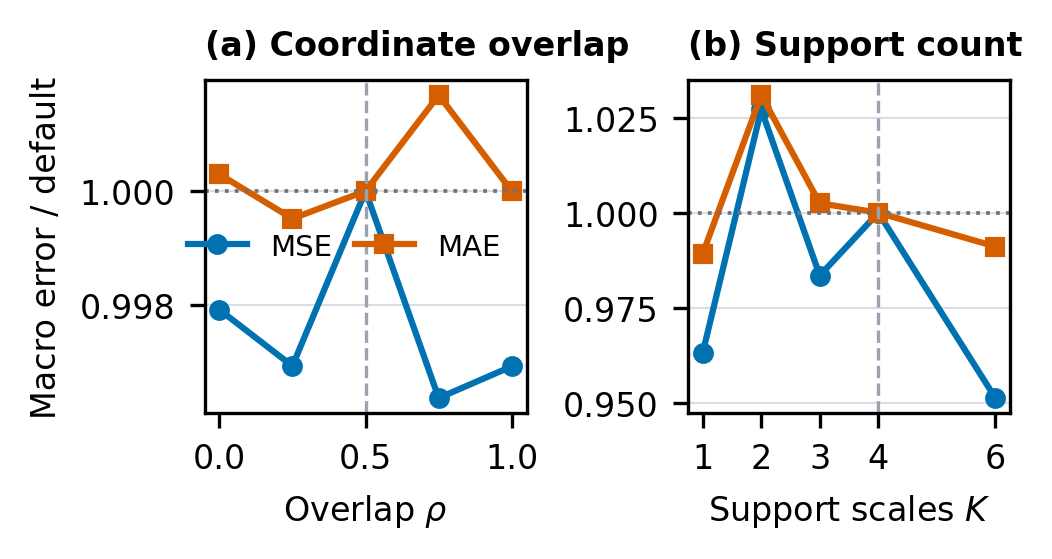
\includegraphics[width=.62\textwidth]{figures/final/mesa_fig4_v675_method_sensitivity.png}
\caption{Sensitivity to DCT overlap $\rho$ and causal support count $K$.}
\label{fig:v675-method-app}
\end{figure}

\begin{table}[H]
\centering
\setlength{\tabcolsep}{5pt}
\caption{Validation MSE/MAE for the method-parameter sweeps. Lower is better.}
\label{tab:v675-method-sensitivity}
\begin{tabular}{@{}lccccc@{}}
\toprule
\multicolumn{6}{c}{DCT overlap $\rho$} \\
\midrule
Dataset & 0 & 0.25 & 0.5 & 0.75 & 1 \\
\midrule
HumanActivity & 0.0420/0.1152 & 0.0421/0.1155 & 0.0422/0.1153 & 0.0422/0.1165 & 0.0422/0.1159 \\
MHEALTH & 0.6189/0.3776 & 0.6165/0.3765 & 0.6238/0.3780 & 0.6153/0.3764 & 0.6168/0.3766 \\
OPPORTUNITY & 0.9349/0.5309 & 0.9337/0.5299 & 0.9329/0.5301 & 0.9323/0.5303 & 0.9324/0.5303 \\
PAMAP2 & 0.4921/0.3673 & 0.4916/0.3668 & 0.4920/0.3666 & 0.4919/0.3666 & 0.4906/0.3660 \\
\midrule
\multicolumn{6}{c}{Causal support count $K$} \\
\midrule
Dataset & 1 & 2 & 3 & 4 & 6 \\
\midrule
HumanActivity & 0.0428/0.1169 & 0.0427/0.1164 & 0.0424/0.1154 & 0.0422/0.1153 & 0.0419/0.1153 \\
MHEALTH & 0.5845/0.3694 & 0.6378/0.3895 & 0.5833/0.3769 & 0.6238/0.3780 & 0.5208/0.3606 \\
OPPORTUNITY & 0.9131/0.5198 & 0.9163/0.5208 & 0.8990/0.5152 & 0.9329/0.5301 & 0.9343/0.5343 \\
PAMAP2 & 0.4533/0.3611 & 0.5366/0.4037 & 0.5063/0.3813 & 0.4920/0.3666 & 0.4791/0.3676 \\
\bottomrule
\end{tabular}
\end{table}


Table~\ref{tab:v675-method-sensitivity} gives the unnormalized validation
errors represented by Figure~\ref{fig:v675-method-app}.

The overlap sweep is flat: all macro MSE points lie within $0.36\%$ and all
macro MAE points within $0.17\%$ of the deployed $\rho=0.5$. The support-count
sweep is intentionally more diagnostic. HumanActivity improves gradually with
additional supports, MHEALTH favors six, OPPORTUNITY favors three, and PAMAP2
favors one in this validation run. The main benchmark keeps one shared $K=4$
configuration, so these values characterize sensitivity rather than define a
per-dataset model-selection rule.

\section{Efficiency Profile}

Figure~\ref{fig:v665-efficiency-app} and
Table~\ref{tab:v665-efficiency} report the exact single-GPU profile used in
the main paper. Parameters and MACs describe model size and arithmetic cost;
peak allocated memory and per-step time are measured with a common batch size
of 4 on MHEALTH. All six methods are profiled under this setting.

\begin{figure}[H]
\centering
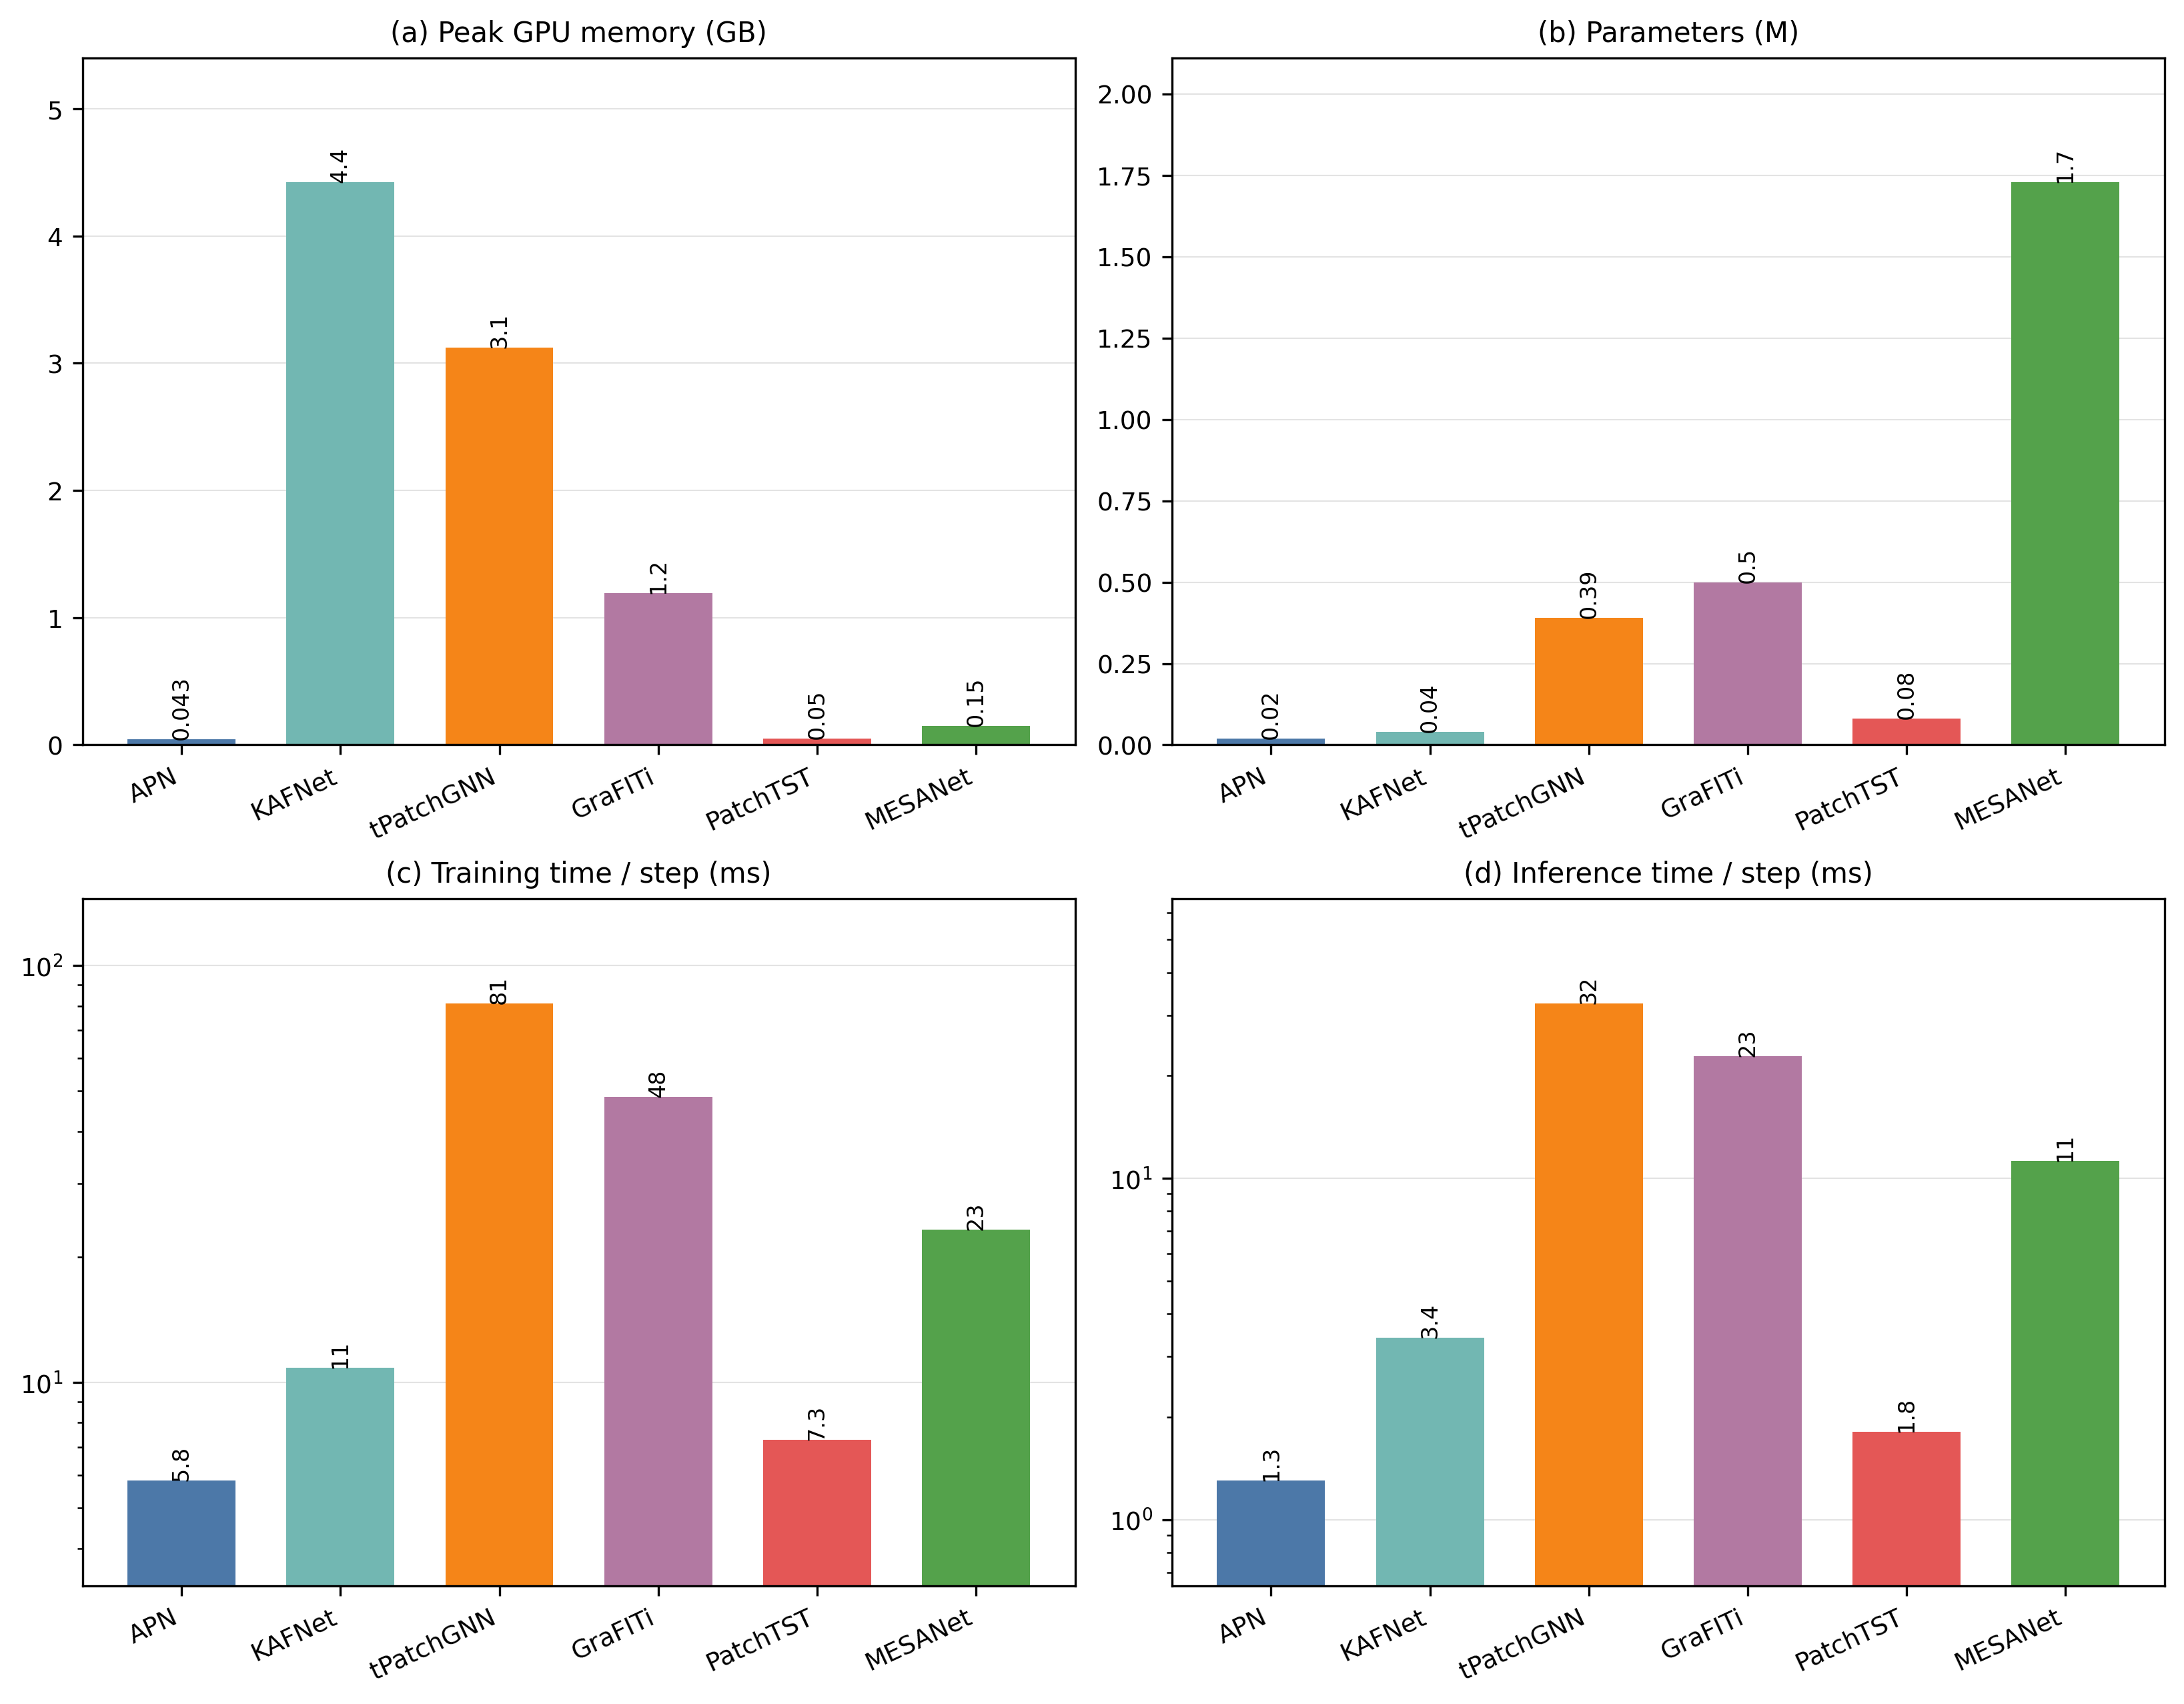
\includegraphics[width=.82\textwidth]{figures/final/mesa_fig4_v665_efficiency_wide_grid.png}
\caption{Computational efficiency on MHEALTH at batch size 4. Training and
inference panels use logarithmic vertical axes.}
\label{fig:v665-efficiency-app}
\end{figure}

\begin{table}[t]
\centering
\setlength{\tabcolsep}{2.2pt}
\caption{Efficiency on MHEALTH (batch size 4; lower is better). Par./MACs/Mem. use M/G/GB; Tr./Inf. use ms.}
\label{tab:v665-efficiency}
\begin{tabular}{@{}lrrrrr@{}}
\toprule
Method & Par. & MACs & Mem. & Tr. & Inf. \\
\midrule
APN       & \textbf{.021} & .017 & \textbf{.043} & \textbf{5.81} & \textbf{1.30} \\
KAFNet    & .038 & \textbf{.011} & 4.425 & 10.83 & 3.41 \\
tPatchGNN & .391 & .367 & 3.121 & 81.04 & 32.42 \\
GraFITi   & .498 & 3.670 & 1.192 & 48.35 & 22.77 \\
PatchTST  & .077 & .020 & .050 & 7.27 & 1.81 \\
MESANet   & 1.733 & .305 & .151 & 23.28 & 11.24 \\
\bottomrule
\end{tabular}
\end{table}


\section{Proofs}

\paragraph{Proposition 1.}
For $x'=ax+c$ with $a>0$, the observed-history mean and scale become
$\mu'=a\mu+c$ and $s'=as$ when $\epsilon=0$ and the scale floor is inactive.
Consequently $z'=m(x'-\mu')/s'=z$. Every timestamp, mask, support statistic,
ordered canonical field, token, and normalized forecast is unchanged. Affine
restoration gives $\widehat y'=\mu'+s'\widehat z=a\widehat y+c$. With finite
$\epsilon$ and variance $v>0$, the scale departure is
\begin{equation}
\left|\sqrt{a^2v+\epsilon}-a\sqrt{v+\epsilon}\right|
=\frac{\epsilon|1-a^2|}
{\sqrt{a^2v+\epsilon}+a\sqrt{v+\epsilon}},
\end{equation}
which vanishes relative to signal scale as $\epsilon/v\rightarrow0$.

\paragraph{Proposition 2.}
The predictor measurable with respect to $(Q,S)$ uses conditional mean
$\boldsymbol\mu_r$ in state $s_r$. A $Q$-measurable predictor on the slice
$Q=q$ must use
$\bar{\boldsymbol\mu}=\pi\boldsymbol\mu_1+(1-\pi)\boldsymbol\mu_2$.
Conditional-variance decomposition gives
\begin{align}
&\pi\|\boldsymbol\mu_1-\bar{\boldsymbol\mu}\|_2^2
+(1-\pi)\|\boldsymbol\mu_2-\bar{\boldsymbol\mu}\|_2^2 \\
&\qquad=\pi(1-\pi)\|\boldsymbol\mu_1-\boldsymbol\mu_2\|_2^2.
\end{align}
This is precisely the excess Bayes risk induced by the collision.

\paragraph{Proposition 3.}
Conditional-variance decomposition first gives
\begin{equation}
\mathcal R(f)-\mathcal R^*
=\mathbb E\|\boldsymbol\mu(X)-f(X)\|_2^2.
\end{equation}
The ranges of $P_B$ and $I-P_B$ are orthogonal. Substituting
$f=\boldsymbol\ell+(I-\rho P_B)\mathbf r$ and using
$P_B\boldsymbol\ell=\boldsymbol\ell$ therefore splits the squared norm into
the low-subspace and orthogonal-residual terms stated in Proposition 3.
Applying $\|a+b\|_2^2\leq2\|a\|_2^2+2\|b\|_2^2$ to the first term yields
the stated upper bound.

For the separation identities, $\mathbf P_B$ is an orthogonal projector, so
$\mathbf P_B^2=\mathbf P_B$ and $\mathbf P_B^\top=\mathbf P_B$. Therefore
\begin{equation}
\mathbf P_B(\mathbf I-\rho\mathbf P_B)\mathbf h^{\rm raw}
=(1-\rho)\mathbf P_B\mathbf h^{\rm raw},
\end{equation}
which gives the leakage identity. The modification is
$-\rho\mathbf P_B\mathbf h^{\rm raw}$, whose norm gives the distortion
identity.

\paragraph{Operator complexity.}
Let $N_{\rm obs}$ be the number of observed scalar history entries, $P$ the
number of patches, $D$ the number of variables, and $d$ the hidden width.
The causal support bank costs $O(KN_{\rm obs}+KPDd^2)$, ordered waveform
encoding costs $O(PDSd)$ for $S$ positions per patch, and the two variable
attention operators cost $O(PD^2d)$. The forecast heads and separation cost
$O(DPd(H+R)+DHR)$. Memory is $O(PDd+DH)$ apart from attention activations.

\section{Reproducibility Commands}

The archived six-trial search and run-5401 confirmation are regenerated by:
\begin{verbatim}
python scripts/run_mesa_equal_hpo.py \
  --datasets HumanActivity,MHEALTH,OPPORTUNITY,PAMAP2,USCHAD,REALDISP \
  --models APN,KAFNet,GraFITi,tPatchGNN,PatchTST,MESANet \
  --search_epochs 20 --confirm_epochs 20 --patience 5 \
  --confirm_seeds 5401 --mae_weight 0.5 \
  --wearable_split_protocol subject_heldout \
  --wearable_mask_protocol real_missing_only_if_available \
  --mesa_ablation aa_no_q_graph_no_prob_waveform_token_parallel_\
dct_dual_coordinate_dct_dual_rho_half_dct_dual_no_causal \
  --root storage/results_mesa_equal_hpo \
  --prefix mesa_equal_hpo
\end{verbatim}

After configuration freezing, the five-run public rows and fixed final model
are generated without test-set reselection by:
\begin{verbatim}
python scripts/run_mesa_v668_frontier_repeated.py \
  --seeds 5402,5403,5404,5405 --epochs 20 --patience 6 \
  --root storage/results_mesa_v668_frontier_repeated \
  --prefix mesa_v668_frontier
python scripts/run_mesa_v671_final_revision.py \
  --variants fixed_rho_half,shared_transfer_matched,random_basis \
  --parallel 4 --epochs 20 --patience 6
python scripts/summarize_mesa_v671_validation_frozen.py
python scripts/summarize_mesa_v671_controls.py
python scripts/analyze_mesa_v671_dual_coordinate_diagnostic.py
python scripts/run_mesa_v672_final_loso.py --fold_parallel 4
python scripts/summarize_mesa_v672_final_loso.py
python scripts/run_mesa_v673_mask_robustness.py --parallel 4
python scripts/summarize_mesa_v673_mask_robustness.py
python scripts/run_mesa_v671_final_revision.py \
  --variants fixed_rho_half,no_multiresolution_fixed,no_affine_anchor_fixed \
  --parallel 2 --epochs 20 --patience 6 \
  --prefix mesa_v674_fixed_components \
  --root storage/results_mesa_v674_fixed_component_ablation
\end{verbatim}

The method-parameter sensitivity is generated by
\begin{verbatim}
python scripts/run_mesa_v675_method_sensitivity.py \
  --root storage/v675 --search_seed 5399 \
  --search_epochs 20 --patience 6 --parallel 3
python scripts/plot_mesa_v675_method_sensitivity.py
\end{verbatim}
The efficiency profile and both PDF/PNG layouts are generated by
\begin{verbatim}
python scripts/run_release_v553_mesa_efficiency.py \
  --dataset MHEALTH \
  --models APN,KAFNet,tPatchGNN,GraFITi,PatchTST,MESANet \
  --batch_size 4 --run_seed 5401 --epochs 4 --patience 2 \
  --mesa_variant mesanet_fixed_dual_coordinate \
  --mesa_width_multiplier 1.5 \
  --wearable_mask_protocol real_missing_only_if_available \
  --root storage/results_mesa_v666_efficiency \
  --summary_name mesa_v666_efficiency_b4.csv \
  --figure_name mesa_fig4_v665_efficiency
\end{verbatim}
\begin{sloppypar}
Figure~2 is editable in
\path{figures/final/mesa_fig2_v676.drawio}. Current paper inputs are
\path{results_mesa_equal_hpo/_summary/equal_hpo_validation_trials.csv},
\path{results_mesa_equal_hpo/_summary/equal_hpo_test_runs.csv},
\path{results_mesa_v671_validation_frozen/_summary/validation_frozen_five_run.csv},
\path{results_mesa_v671_validation_frozen/_summary/validation_frozen_comparators.csv},
\path{results_mesa_v667_final_ablation/_summary/final_evidence_runs.csv},
\path{results_mesa_v671_final_revision/_summary/final_revision_runs.csv}, and
\path{results_mesa_v674_fixed_component_ablation/_summary/final_revision_runs.csv}.
The method-sensitivity source is
\path{storage/v675/_summary/method_sensitivity.csv}. JSON command manifests
stored beside the result roots record every expanded training invocation.
\end{sloppypar}
\end{document}
